\documentclass[12pt,a4paper]{article}
\usepackage[a4paper,top=12mm,bottom=14mm,left=15mm,right=15mm]{geometry}
\usepackage[T1]{fontenc}
\usepackage{amsmath}
\usepackage{amssymb}
\usepackage{enumitem}
\usepackage{multicol}
\usepackage{xcolor}
\usepackage{tikz}
\usepackage{pgfplots}
\pgfplotsset{compat=1.18}
\usepackage[most]{tcolorbox}
\usetikzlibrary{arrows.meta}

% ================================================================
% Currency conversion graphs.
%
% An extension sheet for ratio and proportion, designed to be worked
% through alone. It starts from the idea that a conversion graph
% with no fee is a straight line through the origin, and builds in
% four stages: matching lines to currencies by their steepness,
% measuring steepness as a gradient, adding a flat fee to give a
% y-intercept, and finding where two bureaux give the same amount by
% solving simultaneous equations. The sheet ends with open problems.
% Part 1 has no worked example: pupils find the link between the
% exchange rate and the steepness of a line for themselves in Q1,
% and then use it in Q2 and Q3.
% Pounds are on the x-axis throughout, apart from Q6, which turns the
% graph around on purpose. Answers are on the last page so that
% pupils can check each part before going on.
%
% The exchange rates are rounded versions of real rates, chosen so
% that every line passes through grid points and every step of the
% algebra comes out exactly.
%
% The sheet is written on, so every question is followed by a
% working area. The \newpage commands in the body are placed so
% that no question is split across the fold.
% ================================================================

\pagestyle{empty}
\linespread{1.15}\selectfont
\setlength{\parskip}{5pt}
\renewcommand{\arraystretch}{1.3}
\setlist[enumerate,1]{label=\textbf{Q\arabic*.}, leftmargin=*, itemsep=10pt, topsep=6pt, parsep=4pt}
\setlist[enumerate,2]{label=(\alph*), leftmargin=*, itemsep=8pt, topsep=5pt, parsep=3pt}
\setlength{\multicolsep}{4pt}
\setlength{\parindent}{0pt}

\newcommand{\ansline}[1][2.2cm]{\underline{\hspace{#1}}}
\newcommand{\zl}{z\l{}oty}

% A worked example: the method shown in full before it is practised.
% The boxes are drawn in pale tints, with a pale title bar, so that
% the printed sheet uses little toner.
\newtcolorbox{wex}[1]{colback=blue!2,colframe=blue!30,boxrule=0.6pt,
  colbacktitle=blue!8,coltitle=blue!50!black,
  left=6pt,right=6pt,top=4pt,bottom=5pt,
  title={\bfseries\small Worked example: #1},fonttitle=\small,
  toptitle=1pt,bottomtitle=1pt}

% The idea a section is built on, stated once and boxed.
\newtcolorbox{keyidea}{colback=orange!3,colframe=orange!35,boxrule=0.6pt,
  left=6pt,right=6pt,top=4pt,bottom=4pt}

% The section headings, kept tight so the parts do not eat the page.
\newcommand{\heading}[1]{%
  \vspace{2pt}
  {\color{blue!45!black}\rule{\linewidth}{1pt}}\\[1pt]
  {\large\bfseries #1}\\[-6pt]
  {\color{blue!45!black}\rule{\linewidth}{0.4pt}}
  \vspace{2pt}}
\newcommand{\parttitle}[2]{\heading{Part #1: #2}}

% ----------------------------------------------------------------
% Conversion graphs.
%
% Every graph uses the convgraph style: pounds along the x-axis,
% a light grid on the minor ticks and a darker one on the major
% ticks, and room outside the axes for the letter at the end of
% each line. The size and the scales are given at each graph.
% Graphs with a fee go below zero, so they use feegraph instead,
% which moves the x-axis up to y = 0.
\pgfplotsset{
  convgraph/.style={
    scale only axis,
    axis lines=left,
    axis line style={-},
    grid=both,
    major grid style={gray!55,line width=0.3pt},
    minor grid style={gray!20,line width=0.2pt},
    tick label style={font=\scriptsize},
    label style={font=\small},
    xlabel={Pounds (\pounds)},
    enlargelimits=false,
    clip=false,
    every axis plot/.append style={very thick,samples=2},
  },
  feegraph/.style={
    convgraph,
    axis x line=middle,
    axis y line=left,
    xlabel style={at={(rel axis cs:0.5,0)},anchor=north,yshift=-3pt},
  },
}
% The letter naming a line, written just past its end.
\newcommand{\linename}[1]{node[pos=1,right,font=\small\bfseries,text=black]{#1}}

\definecolor{lineA}{RGB}{0,90,170}
\definecolor{lineB}{RGB}{200,60,20}
\definecolor{lineC}{RGB}{20,130,60}

\begin{document}

\begin{center}
  {\Large\bfseries Currency Conversion Graphs}\\[8pt]
\end{center}
\vspace{1pt}

\begin{keyidea}
\small
A \textbf{bureau de change} is a place where money is changed from one
currency into another. The \textbf{exchange rate} is the amount of the other
currency that \pounds1 buys. When there is no fee, the amount of the other
currency is directly proportional to the number of pounds, so the conversion
graph is a straight line through the origin. Work through this sheet to find
out how the steepness and the position of the line describe the exchange.

\smallskip
The exchange rates in this sheet are rounded. Real exchange rates change every
day.
\end{keyidea}

\parttitle{1}{Which line shows which currency?}

In every graph in this part, pounds are on the x-axis and the amount of
another currency is on the y-axis. The graphs do not say which currency each
line shows: use the exchange rates in the tables to work it out.

\begin{enumerate}

\item The graph shows three conversion graphs. Each line shows one of the
currencies in the table.
\vspace{2pt}

\begin{minipage}[t]{0.52\linewidth}
\centering
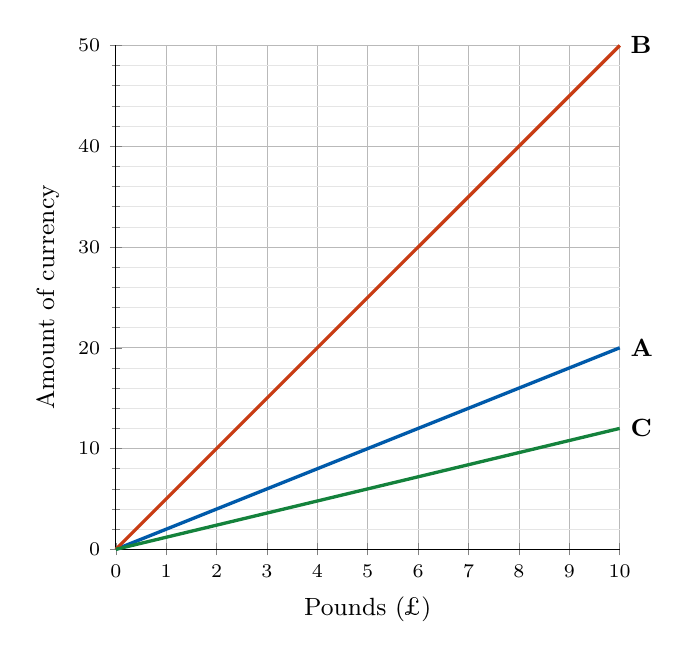
\begin{tikzpicture}[baseline=(current bounding box.north)]
\begin{axis}[convgraph,
    width=6.4cm,height=6.4cm,
    xmin=0,xmax=10,ymin=0,ymax=50,
    xtick distance=1,
    ytick distance=10,minor y tick num=4,
    ylabel={Amount of currency}]
  \addplot[lineA,domain=0:10] {2*x} \linename{A};
  \addplot[lineB,domain=0:10] {5*x} \linename{B};
  \addplot[lineC,domain=0:10] {1.2*x} \linename{C};
\end{axis}
\end{tikzpicture}
\end{minipage}%
\begin{minipage}[t]{0.48\linewidth}
\vspace{6pt}
\begin{tabular}{|l|c|}
\hline
\textbf{Currency} & \textbf{\pounds1 buys}\\
\hline
Euros (\texteuro) & $1.20$\\
\hline
Australian dollars & $2$\\
\hline
Polish \zl{} & $5$\\
\hline
\end{tabular}

\begin{enumerate}
  \item Which line shows Australian dollars?

        Line \ansline[2cm]
\end{enumerate}
\end{minipage}

\begin{enumerate}[start=2]
  \item Explain how you decided which line shows Australian dollars. Use each
        of these words in your answer.

        \begin{center}
        \fbox{\quad\textbf{steeper}\qquad\textbf{steepest}\qquad
        \textbf{less steep}\qquad\textbf{least steep}\quad}
        \end{center}

        \vspace{6em}
  \item Use the graph to convert \pounds7 into Australian dollars.
        \hfill \ansline[2.5cm] Australian dollars
  \item Use the graph to convert \texteuro6 into pounds.
        \hfill \pounds\ansline[2.5cm]
\end{enumerate}

\newpage

\item The table shows how much of four currencies \pounds1 buys. The four
conversion graphs are drawn on the same axes, with pounds on the x-axis.
\vspace{2pt}

\begin{minipage}[t]{0.42\linewidth}
\vspace{4pt}
\begin{tabular}{|l|c|}
\hline
\textbf{Currency} & \textbf{\pounds1 buys}\\
\hline
Norwegian kroner & $13.50$\\
\hline
Indian rupees & $115$\\
\hline
Hong Kong dollars & $10.50$\\
\hline
Mexican pesos & $25$\\
\hline
\end{tabular}
\end{minipage}%
\begin{minipage}[t]{0.58\linewidth}
\centering
\begin{tikzpicture}[baseline=(current bounding box.north),font=\small]
  \draw[-{Stealth[length=2mm]}] (0,0) -- (8,0)
    node[anchor=north east,yshift=-2pt]{Pounds (\pounds)};
  \draw[-{Stealth[length=2mm]}] (0,0) -- (0,7)
    node[above]{Amount of currency};
  \node[below left] at (0,0) {$0$};
\end{tikzpicture}
\end{minipage}

\begin{enumerate}
  \item Sketch the four conversion graphs on the axes. The axes do not need a
        scale, but the lines must be in the right order of steepness. Label
        each line with its currency.
  \item Explain why every one of the four lines passes through the origin.

        \vspace{8em}
\end{enumerate}

\newpage

\item The graph shows three more conversion graphs, but this time there are
five currencies in the table. Two of the currencies do not have a line.
\vspace{2pt}

\begin{minipage}[t]{0.52\linewidth}
\centering
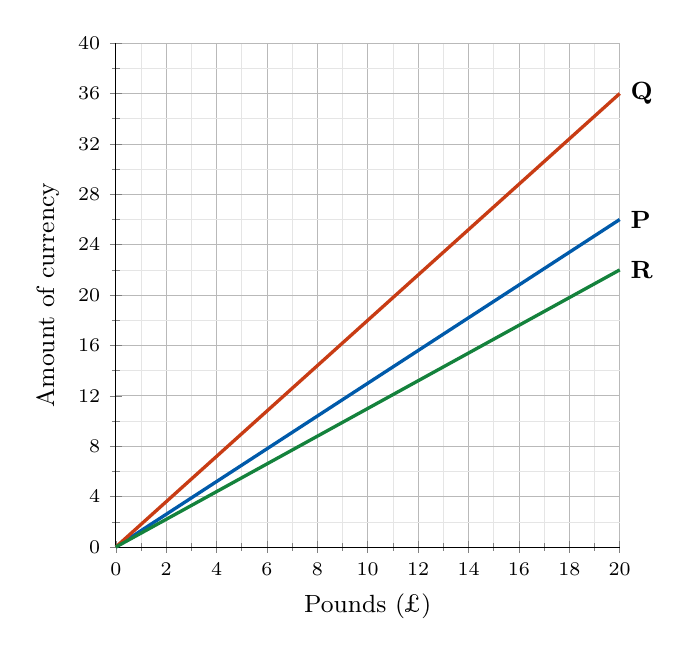
\begin{tikzpicture}[baseline=(current bounding box.north)]
\begin{axis}[convgraph,
    width=6.4cm,height=6.4cm,
    xmin=0,xmax=20,ymin=0,ymax=40,
    xtick distance=2,minor x tick num=1,
    ytick distance=4,minor y tick num=1,
    ylabel={Amount of currency}]
  \addplot[lineA,domain=0:20] {1.3*x} \linename{P};
  \addplot[lineB,domain=0:20] {1.8*x} \linename{Q};
  \addplot[lineC,domain=0:20] {1.1*x} \linename{R};
\end{axis}
\end{tikzpicture}
\end{minipage}%
\begin{minipage}[t]{0.48\linewidth}
\vspace{6pt}
\begin{tabular}{|l|c|}
\hline
\textbf{Currency} & \textbf{\pounds1 buys}\\
\hline
US dollars & $1.30$\\
\hline
Swiss francs & $1.10$\\
\hline
Canadian dollars & $1.80$\\
\hline
Singapore dollars & $1.70$\\
\hline
New Zealand dollars & $2.20$\\
\hline
\end{tabular}
\end{minipage}

\begin{enumerate}
  \item Write down the currency shown by each line.

        Line P: \ansline[3.5cm] \quad Line Q: \ansline[3.5cm] \quad
        Line R: \ansline[3.5cm]

        \vspace{5em}
  \item Draw the lines for Singapore dollars and New Zealand dollars on the
        graph. Label each line with its currency.
  \item Sam says: ``Line Q is the steepest line, so it must show New Zealand
        dollars, because \pounds1 buys more New Zealand dollars than any other
        currency in the table.'' Explain why Sam is wrong.

        \vspace{7em}
\end{enumerate}

\end{enumerate}

\newpage

\parttitle{2}{Measuring steepness with the gradient}

To compare steepness exactly, we measure it with a number called the
\textbf{gradient}. The gradient of a straight line is how far the line rises
for every $1$ unit it moves to the right:
\[
  \text{gradient}=\frac{\text{change in } y}{\text{change in } x}
\]
In a conversion graph, $x$ stands for the number of pounds and $y$ stands for
the amount of the other currency. Moving $1$ unit to the right means adding
\pounds1, so the gradient is the exchange rate. A straight line through the
origin with gradient $m$ has the equation $y=mx$ (remember $mx=m\times x$).

\begin{wex}{find the gradient of the Moroccan dirham line}
\small
\begin{minipage}[t]{0.40\linewidth}
\centering
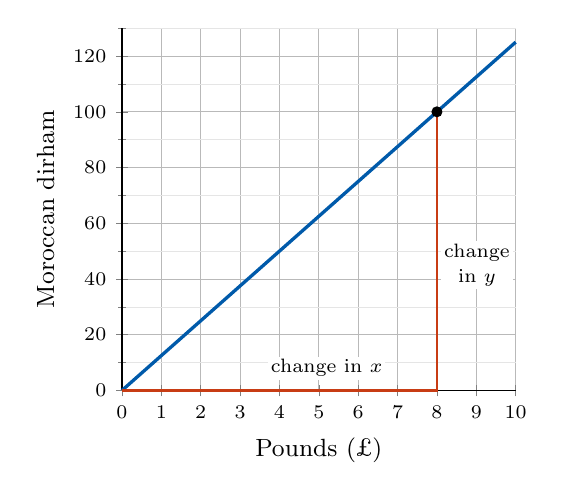
\begin{tikzpicture}[baseline=(current bounding box.north)]
\begin{axis}[convgraph,
    width=5cm,height=4.6cm,
    xmin=0,xmax=10,ymin=0,ymax=130,
    xtick distance=1,
    ytick distance=20,minor y tick num=1,
    ylabel={Moroccan dirham}]
  \addplot[lineA,domain=0:10] {12.5*x};
  \draw[lineB,thick] (axis cs:0,0) -- (axis cs:8,0) -- (axis cs:8,100);
  \fill (axis cs:8,100) circle (2pt);
  \node[font=\scriptsize,fill=white,inner sep=1pt] at (axis cs:5.2,8)
    {change in $x$};
  \node[font=\scriptsize,anchor=west,fill=white,inner sep=1pt] at
    (axis cs:8.1,45) {\shortstack{change\\in $y$}};
\end{axis}
\end{tikzpicture}
\end{minipage}%
\begin{minipage}[t]{0.60\linewidth}
\vspace{0pt}
\begin{tabular}{@{}l@{\hspace{0.8em}}l@{}}
\textbf{Two points on the line} & $(0,0)$ and $(8,100)$\\
\textbf{Change in $x$} & $8-0=8$\\
\textbf{Change in $y$} & $100-0=100$\\
\textbf{Gradient} & $100\div8=12.5$\\
\textbf{Equation of the line} & $y=12.5x$\\
\textbf{What the gradient means} & \pounds1 buys $12.5$ dirham
\end{tabular}
\end{minipage}
\end{wex}

\begin{enumerate}[resume]

\item The graph shows the conversion graph for South African rand. Fill in the
gaps to find its gradient.
\vspace{2pt}

\begin{minipage}[t]{0.40\linewidth}
\centering
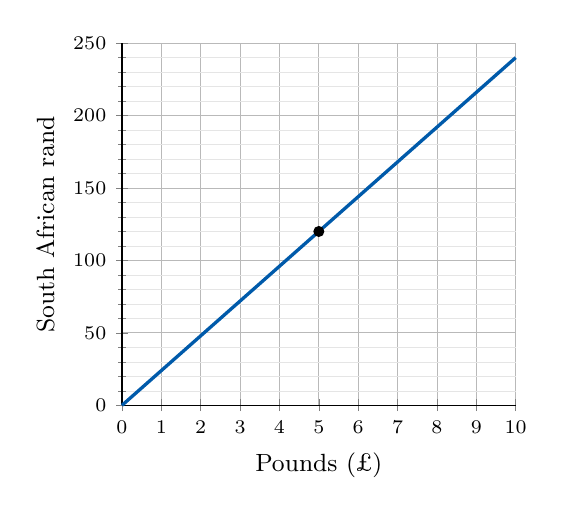
\begin{tikzpicture}[baseline=(current bounding box.north)]
\begin{axis}[convgraph,
    width=5cm,height=4.6cm,
    xmin=0,xmax=10,ymin=0,ymax=250,
    xtick distance=1,
    ytick distance=50,minor y tick num=4,
    ylabel={South African rand}]
  \addplot[lineA,domain=0:10] {24*x};
  \fill (axis cs:5,120) circle (2pt);
\end{axis}
\end{tikzpicture}
\end{minipage}%
\begin{minipage}[t]{0.60\linewidth}
\vspace{0pt}
\begin{tabular}{@{}l@{\hspace{0.8em}}l@{}}
\textbf{Two points on the line} & $(0,0)$ and $(5,\ansline[1.2cm])$\\[4pt]
\textbf{Change in $x$} & $5-0=\ansline[1.2cm]$\\[4pt]
\textbf{Change in $y$} & $\ansline[1.2cm]-0=\ansline[1.2cm]$\\[4pt]
\textbf{Gradient} & $\ansline[1cm]\div\ansline[1cm]=\ansline[1cm]$\\[4pt]
\textbf{Equation of the line} & $y=\ansline[1.2cm]\,x$\\[4pt]
\textbf{What the gradient means} & \pounds1 buys \ansline[1.2cm] rand
\end{tabular}
\end{minipage}

\newpage

\item The graph shows two conversion graphs. One line shows Japanese yen and
the other shows Pakistani rupees. \pounds1 buys more rupees than yen.
\vspace{2pt}

\begin{center}
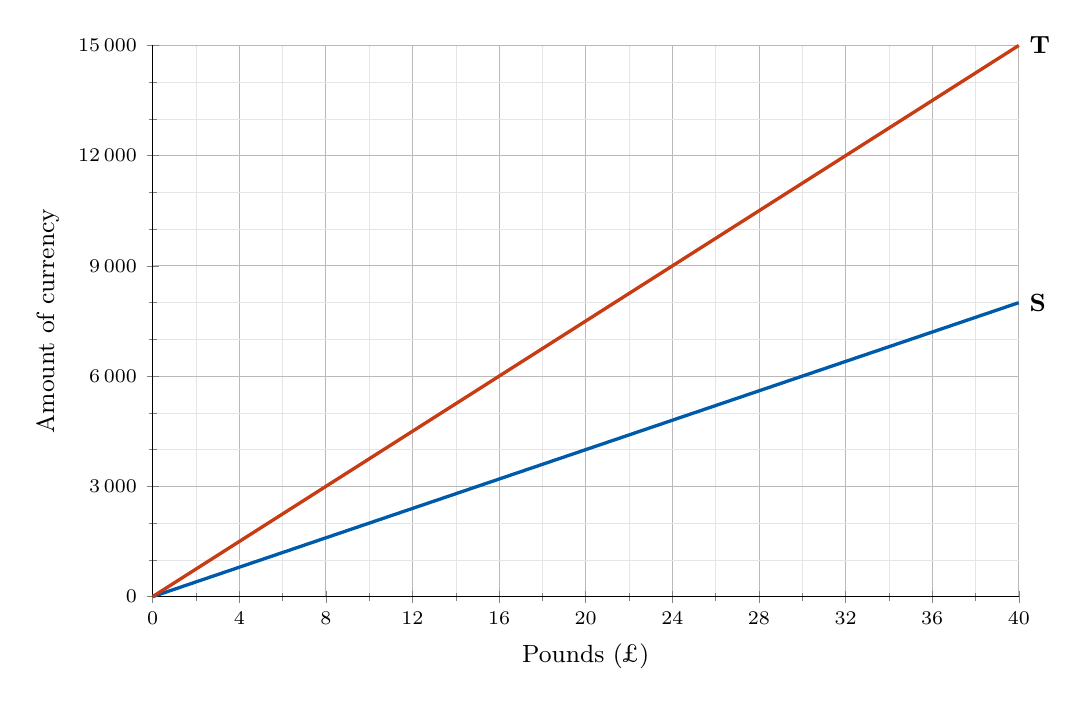
\begin{tikzpicture}
\begin{axis}[convgraph,
    width=11cm,height=7cm,
    xmin=0,xmax=40,ymin=0,ymax=15000,
    xtick distance=4,minor x tick num=1,
    ytick distance=3000,minor y tick num=2,
    scaled y ticks=false,
    yticklabel style={/pgf/number format/1000 sep={\,}},
    ylabel={Amount of currency}]
  \addplot[lineA,domain=0:40] {200*x} \linename{S};
  \addplot[lineB,domain=0:40] {375*x} \linename{T};
\end{axis}
\end{tikzpicture}
\end{center}

\begin{enumerate}
  \item Which line shows Japanese yen? Give a reason for your answer.
        \hfill \ansline[3cm]

        \vspace{3em}
  \item Find the gradient of each line, and write down the equation of each
        line. Set out your working like the worked example.
        \vspace{4pt}

        \begin{minipage}[t]{0.48\linewidth}
        \textbf{Line S}\\[4pt]
        \begin{tabular}{@{}l@{\hspace{0.6em}}l@{}}
        \textbf{Two points on the line} & \ansline[2.4cm]\\[5pt]
        \textbf{Change in $x$} & \ansline[2.4cm]\\[5pt]
        \textbf{Change in $y$} & \ansline[2.4cm]\\[5pt]
        \textbf{Gradient} & \ansline[2.4cm]\\[5pt]
        \textbf{Equation} & \ansline[2.4cm]
        \end{tabular}
        \end{minipage}\hfill
        \begin{minipage}[t]{0.48\linewidth}
        \textbf{Line T}\\[4pt]
        \begin{tabular}{@{}l@{\hspace{0.6em}}l@{}}
        \textbf{Two points on the line} & \ansline[2.4cm]\\[5pt]
        \textbf{Change in $x$} & \ansline[2.4cm]\\[5pt]
        \textbf{Change in $y$} & \ansline[2.4cm]\\[5pt]
        \textbf{Gradient} & \ansline[2.4cm]\\[5pt]
        \textbf{Equation} & \ansline[2.4cm]
        \end{tabular}
        \end{minipage}
  \item The graph stops at \pounds40. Use the equation of line S to convert
        \pounds250 into yen.

        \vspace{3.5em}
  \item Use the equation of line T to convert $30\,000$ rupees into pounds.

        \vspace{4.5em}
\end{enumerate}

\newpage

\item Ola lives in Poland and is visiting London. She draws a conversion graph
the other way round, with Polish \zl{} on the x-axis and pounds on the
y-axis. The exchange rate is \pounds1 $=5$ \zl{}.
\vspace{2pt}

\begin{minipage}[t]{0.62\linewidth}
\centering
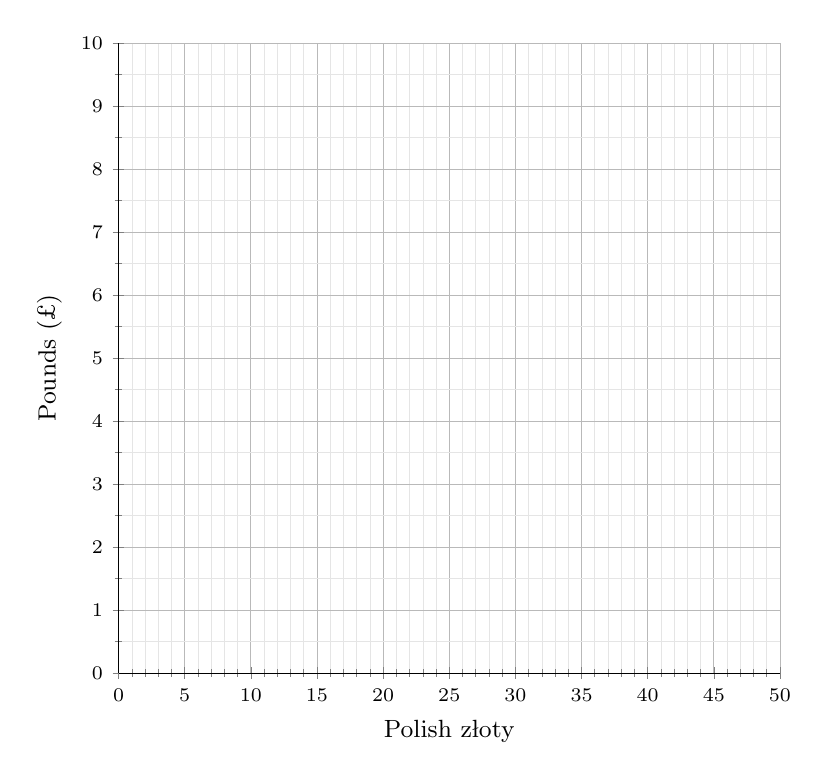
\begin{tikzpicture}[baseline=(current bounding box.north)]
\begin{axis}[convgraph,
    width=8.4cm,height=8cm,
    xmin=0,xmax=50,ymin=0,ymax=10,
    xtick distance=5,minor x tick num=4,
    ytick distance=1,minor y tick num=1,
    xlabel={Polish \zl{}},
    ylabel={Pounds (\pounds)}]
  \addplot[draw=none,domain=0:50] {0};
\end{axis}
\end{tikzpicture}
\end{minipage}%
\begin{minipage}[t]{0.38\linewidth}
\vspace{6pt}
\begin{tabular}{|l|c|c|c|c|}
\hline
\textbf{\zl{}} & $0$ & $10$ & $25$ & $50$\\
\hline
\textbf{\pounds} & $0$ & & & \\
\hline
\end{tabular}

\begin{enumerate}
  \item Complete the table.
  \item Draw the line on the grid.
\end{enumerate}
\end{minipage}

\begin{enumerate}[start=3]
  \item Find the gradient of Ola's line. \hfill \ansline[3cm]

        \vspace{4em}
  \item Explain what the gradient of Ola's line tells her.

        \vspace{6em}
\end{enumerate}

\end{enumerate}

\newpage

\parttitle{3}{Flat fees and the y-intercept}

Some bureaux de change charge a \textbf{flat fee}: a fixed amount that is taken
off every exchange, however much money is changed. The fee is taken off first,
and the pounds that are left are converted.

A straight line with gradient $m$ that crosses the y-axis at $c$ has the
equation $y=mx+c$. The number $c$ is called the \textbf{y-intercept}. For a
bureau with a flat fee, the gradient is still the exchange rate, and the
y-intercept is negative.

\begin{wex}{\pounds5 fee, and \texteuro1.20 for every \pounds1 left}
\small
\begin{minipage}[t]{0.40\linewidth}
\centering
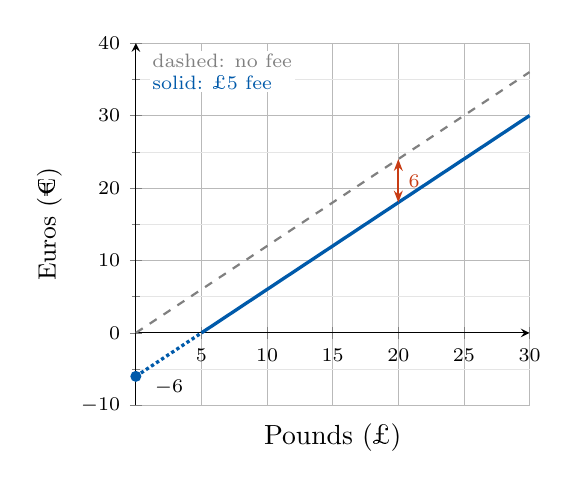
\begin{tikzpicture}[baseline=(current bounding box.north)]
\begin{axis}[feegraph,
    width=5cm,height=4.6cm,
    xmin=0,xmax=30,ymin=-10,ymax=40,
    xtick distance=5,
    ytick distance=10,minor y tick num=1,
    ylabel={Euros (\texteuro)}]
  \addplot[gray,dashed,thick,domain=0:30] {1.2*x};
  \addplot[lineA,densely dotted,domain=0:5] {1.2*x-6};
  \addplot[lineA,domain=5:30] {1.2*x-6};
  \node[font=\scriptsize,anchor=north west,align=left,fill=white,
    inner sep=1pt] at (axis cs:1,39)
    {\textcolor{gray}{dashed: no fee}\\\textcolor{lineA}{solid: \pounds5 fee}};
  \fill[lineA] (axis cs:0,-6) circle (2pt);
  \node[font=\scriptsize,anchor=west,fill=white,inner sep=1pt]
    at (axis cs:1.2,-7.5) {$-6$};
  \draw[{Stealth[length=1.5mm]}-{Stealth[length=1.5mm]},lineB,thick]
    (axis cs:20,24) -- (axis cs:20,18)
    node[midway,right,font=\scriptsize,text=lineB]{$6$};
\end{axis}
\end{tikzpicture}
\end{minipage}%
\begin{minipage}[t]{0.60\linewidth}
\vspace{0pt}
\begin{tabular}{@{}l@{\hspace{0.8em}}l@{}}
\textbf{Pounds converted} & $x-5$\\
\textbf{Euros received} & $y=1.2(x-5)$\\
\textbf{Expand the brackets} & $y=1.2x-6$\\
\textbf{Gradient} & $1.2$, the exchange rate\\
\textbf{y-intercept} & $-6$, the fee of \pounds5\\
 & is worth $1.2\times5=\text{\texteuro}6$
\end{tabular}

\smallskip
The fee line is parallel to the no-fee line, because the exchange rate is the
same. It is \texteuro6 lower at every point, because the fee is worth
\texteuro6. The dotted part of the line is only there to show where the line
meets the y-axis: exchanging less than \pounds5 gives nothing at all.
\end{minipage}
\end{wex}

\begin{enumerate}[resume]

\item A bank charges a flat fee of \pounds10, and gives \$1.30 for every
\pounds1 left. Fill in the gaps to find the equation of its conversion graph.
\vspace{2pt}

\begin{minipage}[t]{0.40\linewidth}
\centering
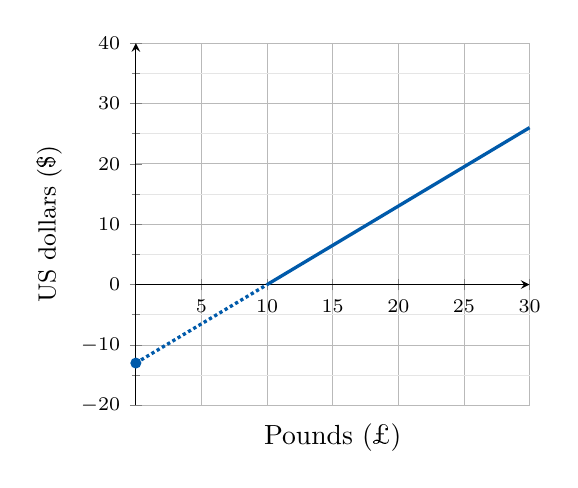
\begin{tikzpicture}[baseline=(current bounding box.north)]
\begin{axis}[feegraph,
    width=5cm,height=4.6cm,
    xmin=0,xmax=30,ymin=-20,ymax=40,
    xtick distance=5,
    ytick distance=10,minor y tick num=1,
    ylabel={US dollars (\$)}]
  \addplot[lineA,densely dotted,domain=0:10] {1.3*x-13};
  \addplot[lineA,domain=10:30] {1.3*x-13};
  \fill[lineA] (axis cs:0,-13) circle (2pt);
\end{axis}
\end{tikzpicture}
\end{minipage}%
\begin{minipage}[t]{0.60\linewidth}
\vspace{0pt}
\begin{tabular}{@{}l@{\hspace{0.8em}}l@{}}
\textbf{Pounds converted} & $x-\ansline[1cm]$\\[4pt]
\textbf{Dollars received} & $y=\ansline[1cm](x-\ansline[1cm])$\\[4pt]
\textbf{Expand the brackets} & $y=\ansline[1cm]\,x-\ansline[1cm]$\\[4pt]
\textbf{Gradient} & \ansline[1cm], the exchange rate\\[4pt]
\textbf{y-intercept} & \ansline[1cm], the fee of \pounds\ansline[0.8cm]\\[4pt]
 & is worth $\ansline[0.8cm]\times\ansline[0.8cm]=\$\ansline[0.8cm]$
\end{tabular}
\end{minipage}

\begin{enumerate}
  \item How many dollars does the bank give for \pounds100?
        \hfill \$\ansline[2.5cm]

        \vspace{3em}
  \item Jo wants to receive exactly \$130. How many pounds must she exchange?
        \hfill \pounds\ansline[2.5cm]

        \vspace{5em}
\end{enumerate}

\newpage

\item The graph shows the conversion graphs for three bureaux de change. As in
the worked example, the dotted part of each line only shows where the line
meets the y-axis.
\vspace{2pt}

\begin{center}
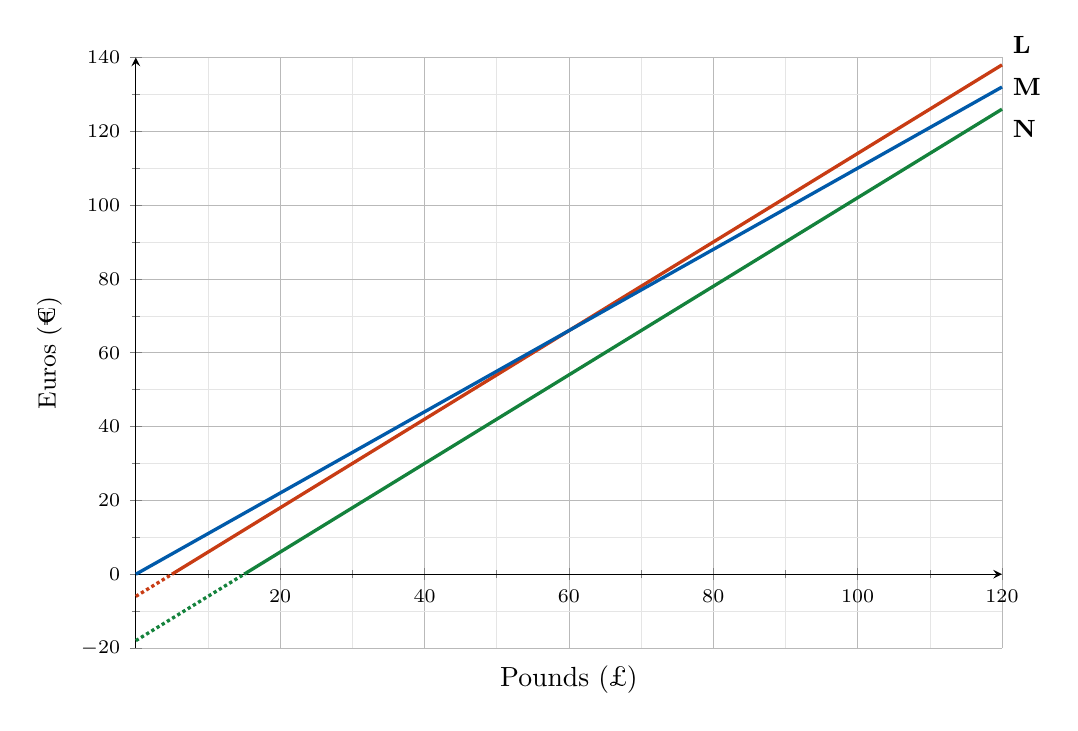
\begin{tikzpicture}
\begin{axis}[feegraph,
    width=11cm,height=7.5cm,
    xmin=0,xmax=120,ymin=-20,ymax=140,
    xtick distance=20,minor x tick num=1,
    ytick distance=20,minor y tick num=1,
    ylabel={Euros (\texteuro)}]
  \addplot[lineB,densely dotted,domain=0:5] {1.2*x-6};
  \addplot[lineB,domain=5:120] {1.2*x-6}
    node[pos=1,above right,font=\small\bfseries,text=black]{L};
  \addplot[lineA,domain=0:120] {1.1*x}
    node[pos=1,right,font=\small\bfseries,text=black]{M};
  \addplot[lineC,densely dotted,domain=0:15] {1.2*x-18};
  \addplot[lineC,domain=15:120] {1.2*x-18}
    node[pos=1,below right,font=\small\bfseries,text=black]{N};
\end{axis}
\end{tikzpicture}
\end{center}

\begin{center}
\begin{tabular}{|l|c|c|c|}
\hline
\textbf{Bureau} & \textbf{Flat fee} & \textbf{Euros for every \pounds1 left}
  & \textbf{Line}\\
\hline
Airport & none & $1.10$ & \\
\hline
High street & \pounds5 & $1.20$ & \\
\hline
Online & \pounds15 & $1.20$ & \\
\hline
\end{tabular}
\end{center}

\begin{enumerate}
  \item Complete the table to match each bureau to its line.
  \item Two of the lines are parallel. Explain why.

        \vspace{3.5em}
  \item Write down the equation of each line in the form $y=mx+c$.

        Line L: \ansline[3cm] \quad Line M: \ansline[3cm] \quad
        Line N: \ansline[3cm]
  \item Lines L and M cross. Use the graph to find the number of pounds where
        they cross, and explain what the crossing point tells you about the
        airport and the high street bureaux.

        \vspace{6em}
\end{enumerate}

\newpage

\item A bureau's conversion graph for Canadian dollars has the equation
\[
  y=1.8x-9
\]
where $x$ is the number of pounds exchanged and $y$ is the number of Canadian
dollars received.
\begin{enumerate}
  \item What is the exchange rate at this bureau? \hfill \ansline[3cm]

        \vspace{2em}
  \item What flat fee does the bureau charge, in pounds? Show how you worked
        it out.

        \vspace{6em}
  \item Explain why this bureau gives no Canadian dollars at all to someone
        who exchanges \pounds5.

        \vspace{6em}
  \item A second bureau has the same exchange rate, but charges a flat fee of
        \pounds10. Write down the equation of its conversion graph, and
        describe how its line compares with the line $y=1.8x-9$.

        \vspace{8em}
\end{enumerate}

\end{enumerate}

\newpage

\parttitle{4}{When do two bureaux give the same amount?}

Where two conversion graphs cross, the two bureaux give the same amount of
currency for the same number of pounds. To find the crossing point exactly, we
set the two expressions for $y$ equal to each other and solve the equation.
Finding the values of $x$ and $y$ that make two equations true at the same time
is called solving \textbf{simultaneous equations}.

\begin{wex}{the airport and the high street bureau from Q8}
\small
\textbf{Airport:} no fee, \texteuro1.10 for every \pounds1, so $y=1.1x$.\\
\textbf{High street:} \pounds5 fee, \texteuro1.20 for every \pounds1 left, so
$y=1.2(x-5)=1.2x-6$.

\smallskip
\begin{center}
\begin{tabular}{|l|c|c|c|c|}
\hline
\textbf{Pounds, $x$} & $0$ & $40$ & $80$ & $120$\\
\hline
\textbf{Airport, $y$} & $0$ & $44$ & $88$ & $132$\\
\hline
\textbf{High street, $y$} & $-6$ & $42$ & $90$ & $138$\\
\hline
\end{tabular}
\end{center}

\begin{minipage}[t]{0.44\linewidth}
\centering
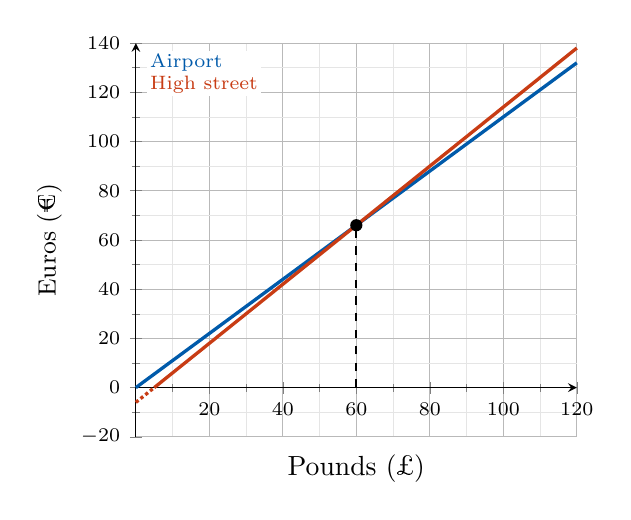
\begin{tikzpicture}[baseline=(current bounding box.north)]
\begin{axis}[feegraph,
    width=5.6cm,height=5cm,
    xmin=0,xmax=120,ymin=-20,ymax=140,
    xtick distance=20,minor x tick num=1,
    ytick distance=20,minor y tick num=1,
    ylabel={Euros (\texteuro)}]
  \addplot[lineA,domain=0:120] {1.1*x};
  \addplot[lineB,densely dotted,domain=0:5] {1.2*x-6};
  \addplot[lineB,domain=5:120] {1.2*x-6};
  \draw[dashed,thick] (axis cs:60,0) -- (axis cs:60,66);
  \fill (axis cs:60,66) circle (2.2pt);
  \node[font=\scriptsize,anchor=north west,align=left,fill=white,
    inner sep=1pt] at (axis cs:3,137)
    {\textcolor{lineA}{Airport}\\\textcolor{lineB}{High street}};
\end{axis}
\end{tikzpicture}
\end{minipage}%
\begin{minipage}[t]{0.56\linewidth}
\vspace{0pt}
The high street line is below the airport line at \pounds40 and above it at
\pounds80, so the lines cross between \pounds40 and \pounds80.

\smallskip
\begin{tabular}{@{}l@{\hspace{0.8em}}l@{}}
\textbf{Same amount when} & $1.1x=1.2x-6$\\
\textbf{Subtract $1.1x$ from both sides} & $0=0.1x-6$\\
\textbf{Add $6$ to both sides} & $6=0.1x$\\
\textbf{Multiply both sides by $10$} & $60=x$\\
\textbf{Euros received} & $y=1.1\times60=66$
\end{tabular}
\end{minipage}

\smallskip
Both bureaux give \texteuro66 for \pounds60. For less than \pounds60 the
airport gives more euros, because its line is higher. For more than \pounds60
the high street bureau gives more euros, because its line is steeper and is
now the higher line.
\end{wex}

\begin{enumerate}[resume]

\item Use the worked example to answer these.
\begin{enumerate}
  \item How many euros does each bureau give for \pounds30? Which bureau gives
        more?

        \vspace{4em}
  \item How many euros does each bureau give for \pounds200? Which bureau
        gives more, and how many more?

        \vspace{4em}
  \item Once the lines have crossed, the difference between the two bureaux
        gets bigger as the number of pounds goes up. Use the gradients of the
        two lines to explain why.

        \vspace{5em}
\end{enumerate}

\newpage

\item An airport bureau and a bureau in town both change pounds into Polish
\zl{}. Fill in the gaps in the equations, the table and the working, as in the
worked example.

\medskip
\textbf{Airport:} no fee, $4.50$ \zl{} for every \pounds1, so
$y=\ansline[1.2cm]\,x$.\\[4pt]
\textbf{Town:} \pounds3 fee, $5$ \zl{} for every \pounds1 left, so
$y=5(x-\ansline[1cm])=\ansline[1cm]\,x-\ansline[1cm]$.

\smallskip
\begin{center}
\begin{tabular}{|l|c|c|c|c|}
\hline
\textbf{Pounds, $x$} & $0$ & $20$ & $40$ & $60$\\
\hline
\textbf{Airport, $y$} & $0$ & \hspace{1.2cm} & \hspace{1.2cm} & \hspace{1.2cm}\\
\hline
\textbf{Town, $y$} & & & & \\
\hline
\end{tabular}
\end{center}

\begin{minipage}[t]{0.42\linewidth}
\centering
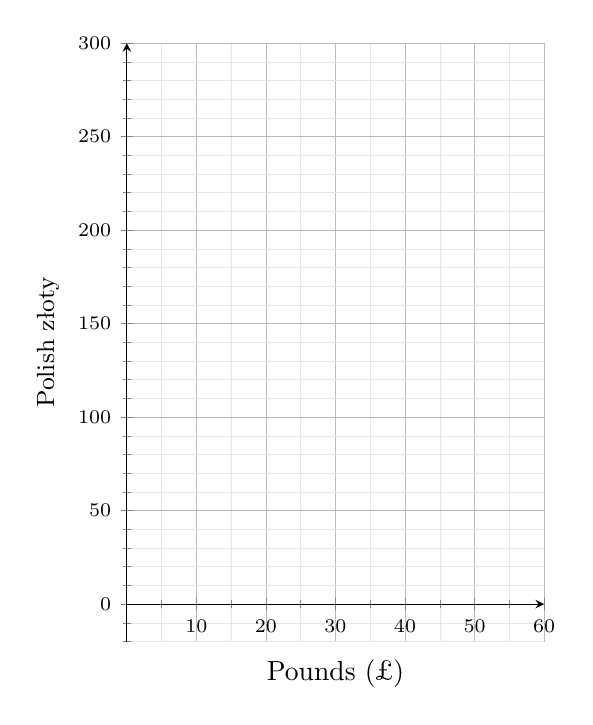
\begin{tikzpicture}[baseline=(current bounding box.north)]
\begin{axis}[feegraph,
    width=5.3cm,height=7.6cm,
    xmin=0,xmax=60,ymin=-20,ymax=300,
    xtick distance=10,minor x tick num=1,
    ytick distance=50,minor y tick num=4,
    ylabel={Polish \zl{}}]
  \addplot[draw=none,domain=0:60] {0};
\end{axis}
\end{tikzpicture}
\end{minipage}%
\begin{minipage}[t]{0.58\linewidth}
\vspace{0pt}
The town line is \ansline[1.4cm] the airport line at \pounds20 and
\ansline[1.4cm] it at \pounds40, so the lines cross between \pounds20 and
\pounds40.

\smallskip
\begin{tabular}{@{}l@{\hspace{0.5em}}l@{}}
\textbf{Same amount when} & $\ansline[1.2cm]=\ansline[1.4cm]$\\[5pt]
\textbf{Subtract $4.5x$ from both sides} & $0=\ansline[0.8cm]\,x-\ansline[0.8cm]$\\[5pt]
\textbf{Add \ansline[0.8cm] to both sides} & $\ansline[0.8cm]=0.5x$\\[5pt]
\textbf{Multiply both sides by \ansline[0.8cm]} & $\ansline[0.8cm]=x$\\[5pt]
\textbf{Z\l{}oty received} & $y=\ansline[1.6cm]$
\end{tabular}
\end{minipage}

\begin{enumerate}
  \item Draw both lines on the grid, and mark the point where they cross.
  \item Which bureau gives more \zl{} for \pounds20? \hfill \ansline[3cm]
  \item Which bureau gives more \zl{} for \pounds50? \hfill \ansline[3cm]
\end{enumerate}

\newpage

\item The airport bureau gives \$1.15 for every \pounds1 and charges no fee. An
online bureau charges a flat fee of \pounds8 and gives \$1.25 for every
\pounds1 left.
\begin{enumerate}
  \item Write down the equation of each conversion graph.

        \vspace{4em}
  \item Find the number of pounds for which both bureaux give the same number
        of dollars, and how many dollars that is.

        \vspace{9em}
  \item Mia is exchanging \pounds400 for a holiday in New York. Which bureau
        should she use, and how many more dollars will she get?

        \vspace{6em}
\end{enumerate}

\item Two bureaux both charge a flat fee. Bureau E charges \pounds2 and gives
$190$ Japanese yen for every \pounds1 left. Bureau F charges \pounds5 and gives
$200$ yen for every \pounds1 left.
\begin{enumerate}
  \item Show that the equation for Bureau E is $y=190x-380$, and write down
        the equation for Bureau F.

        \vspace{4em}
  \item Find the number of pounds for which both bureaux give the same number
        of yen.

        \vspace{7em}
  \item Kenji has \pounds500 to exchange. Which bureau should he use, and how
        many more yen will he get?

        \vspace{5em}
\end{enumerate}

\end{enumerate}

\newpage

\parttitle{5}{Challenges}

\begin{enumerate}[resume]

\item Two bureaux both charge a flat fee of \pounds5. Bureau G gives
\texteuro1.10 for every \pounds1 left, and Bureau H gives \texteuro1.20 for
every \pounds1 left.
\begin{enumerate}
  \item Write down the equation of each conversion graph, and the y-intercept
        of each line.

        \vspace{4.5em}
  \item Show that both lines cross the x-axis at $x=5$, and explain what this
        point means.

        \vspace{6em}
  \item Tom says: ``If two bureaux charge the same flat fee, the bureau with
        the better exchange rate always gives more euros.'' Use your answers
        to parts (a) and (b) to decide whether Tom is right.

        \vspace{8em}
\end{enumerate}

\item The airport bureau gives \texteuro1.10 for every \pounds1 and charges no
fee. Design a deal for a new bureau, with a flat fee and a better exchange
rate, so that the new bureau and the airport give the same number of euros
when exactly \pounds300 is exchanged. Show that your deal works, and explain
who should use the new bureau rather than the airport.

\vspace{12em}

\newpage

\item Some bureaux charge a \textbf{commission} instead of a flat fee. A
commission is a percentage of the pounds exchanged. Bureau K takes $2\%$
commission, and gives \texteuro1.25 for every \pounds1 left.
\begin{enumerate}
  \item Show that exchanging \pounds100 at Bureau K gives \texteuro122.50.

        \vspace{5em}
  \item Aisha says: ``A commission is a kind of fee, so the line for Bureau K
        crosses the y-axis below zero, like the line for the high street
        bureau.'' Explain whether Aisha is right, and find the gradient of the
        line for Bureau K.

        \vspace{9em}
  \item Is Bureau K better or worse than the high street bureau (\pounds5 fee,
        \texteuro1.20 for every \pounds1 left)? Does your answer depend on how
        many pounds are exchanged? Explain using the equations of the two
        lines.

        \vspace{12em}
\end{enumerate}

\end{enumerate}

\newpage

\heading{Answers}

{\small
\begin{multicols}{2}
\raggedcolumns
\setlength{\parskip}{4pt}

\textbf{Q1.} (a) Line A. \quad
(b) For example: \pounds1 buys more \zl{} than either of the other currencies,
so each \pounds1 adds the most to the \zl{} line, and the \zl{} line is the
steepest line, B. \pounds1 buys the fewest euros, so the euro line is the least
steep line, C. \pounds1 buys $2$ Australian dollars, which is more than
\texteuro1.20 and fewer than $5$ \zl{}, so the Australian dollar line is
steeper than the euro line and less steep than the \zl{} line. That is line A.
\quad
(c) $14$ Australian dollars. \quad
(d) \pounds5, reading from line C.

\textbf{Q2.} (a) From the steepest line to the least steep: Indian rupees
($115$), Mexican pesos ($25$), Norwegian kroner ($13.50$), Hong Kong dollars
($10.50$). \quad
(b) \pounds0 buys none of any currency, so every line passes through $(0,0)$.
The amount of each currency is directly proportional to the number of pounds.

\textbf{Q3.} (a) At \pounds20, line P is at $26$, line Q is at $36$ and line R
is at $22$. $26\div20=1.3$, $36\div20=1.8$ and $22\div20=1.1$, so P shows US
dollars, Q shows Canadian dollars and R shows Swiss francs. \quad
(b) Singapore dollars: a straight line from $(0,0)$ through $(10,17)$ and
$(20,34)$, between lines P and Q. New Zealand dollars: a straight line from
$(0,0)$ through $(10,22)$, which reaches the top of the graph at about
\pounds18. It is steeper than line Q. \quad
(c) Line Q is only the steepest of the three lines that were drawn. Two
currencies in the table had no line, and the New Zealand dollar line from part
(b) is steeper than line Q: at \pounds10 it is at $22$, while line Q is at
$18$.

\textbf{Q4.} $(0,0)$ and $(5,120)$. Change in $x$: $5$. Change in $y$:
$120-0=120$. Gradient: $120\div5=24$. Equation: $y=24x$. \pounds1 buys $24$
rand.

\textbf{Q5.} (a) Line S. \pounds1 buys fewer yen than rupees, so the yen line
is the less steep line. \quad
(b) Line S: for example $(0,0)$ and $(40,8000)$; change in $x$ is $40$, change
in $y$ is $8000$, gradient $8000\div40=200$, so $y=200x$. Line T: for example
$(0,0)$ and $(40,15\,000)$; change in $x$ is $40$, change in $y$ is
$15\,000$, gradient $15\,000\div40=375$, so $y=375x$. \quad
(c) $y=200\times250=50\,000$ yen. \quad
(d) $375x=30\,000$, so $x=30\,000\div375=80$. That is \pounds80.

\textbf{Q6.} (a) \pounds0, \pounds2, \pounds5, \pounds10. \quad
(b) A straight line from $(0,0)$ to $(50,10)$. \quad
(c) $10\div50=0.2$. \quad
(d) $1$ \zl{} is worth \pounds0.20, which is $20$p.

\textbf{Q7.} Pounds converted: $x-10$. Dollars received: $y=1.3(x-10)$.
Expanded: $y=1.3x-13$. Gradient: $1.3$. y-intercept: $-13$, the fee of
\pounds10 is worth $1.3\times10=\$13$. \quad
(a) $1.3\times100-13=\$117$. \quad
(b) $1.3x-13=130$, so $1.3x=143$ and $x=110$. Jo must exchange \pounds110.

\textbf{Q8.} (a) Airport: M. High street: L. Online: N. \quad
(b) Lines L and N both give \texteuro1.20 for every \pounds1 left, so both have
gradient $1.2$. \quad
(c) L: $y=1.2x-6$. \quad M: $y=1.1x$. \quad N: $y=1.2x-18$. \quad
(d) \pounds60. The airport and the high street bureau give the same number of
euros (\texteuro66) for \pounds60. For less than \pounds60 the airport gives
more, and for more than \pounds60 the high street bureau gives more.

\textbf{Q9.} (a) C\$1.80 for every \pounds1. \quad
(b) The fee is worth C\$9, so the fee is $9\div1.8=\text{\pounds}5$. \quad
(c) The whole \pounds5 is taken as the fee, so there are no pounds left to
convert: $1.8\times5-9=0$. \quad
(d) $y=1.8x-18$. The line is parallel to $y=1.8x-9$, because the gradient is
the same, and it is $9$ lower at every point, because its y-intercept is $-18$
instead of $-9$.

\textbf{Q10.} (a) The airport gives $1.1\times30=\text{\texteuro}33$ and
the high street bureau gives $1.2\times30-6=\text{\texteuro}30$, so the
airport gives more. \quad
(b) The airport gives $1.1\times200=\text{\texteuro}220$ and the high street
bureau gives $1.2\times200-6=\text{\texteuro}234$, so the high street bureau
gives \texteuro14 more. \quad
(c) The high street line has gradient $1.2$ and the airport line has
gradient $1.1$, so for every extra \pounds1 the high street bureau gives
\texteuro0.10 more than the airport. After the lines cross at \pounds60,
the difference grows by \texteuro0.10 for every \pounds1: at \pounds200 it
is $0.1\times(200-60)=\text{\texteuro}14$.

\textbf{Q11.} Airport: $y=4.5x$. Town: $y=5(x-3)=5x-15$. Table: airport $0$,
$90$, $180$, $270$; town $-15$, $85$, $185$, $285$. The town line is below the
airport line at \pounds20 and above it at \pounds40. Working:
$4.5x=5x-15$; $0=0.5x-15$; add $15$: $15=0.5x$; multiply by $2$: $30=x$;
$y=4.5\times30=135$. \quad
(a) The lines cross at $(30,135)$. \quad
(b) The airport: $90$ \zl{} against $85$ \zl{}. \quad
(c) The town bureau: $235$ \zl{} against $225$ \zl{}.

\textbf{Q12.} (a) Airport: $y=1.15x$. Online: $y=1.25(x-8)=1.25x-10$. \quad
(b) $1.15x=1.25x-10$, so $10=0.1x$ and $x=100$. Both bureaux give \$115 for
\pounds100. \quad
(c) The online bureau: $1.25\times400-10=\$490$, against
$1.15\times400=\$460$ at the airport. She gets \$30 more.

\textbf{Q13.} (a) E: $y=190(x-2)=190x-380$. F: $y=200(x-5)=200x-1000$. \quad
(b) $190x-380=200x-1000$, so $620=10x$ and $x=62$. Both bureaux give
$11\,400$ yen for \pounds62. \quad
(c) Bureau F: $200\times500-1000=99\,000$ yen, against
$190\times500-380=94\,620$ yen at Bureau E. He gets $4380$ more yen.

\textbf{Q14.} (a) G: $y=1.1(x-5)=1.1x-5.5$, y-intercept $-5.5$. H:
$y=1.2(x-5)=1.2x-6$, y-intercept $-6$. \quad
(b) $1.1\times5-5.5=0$ and $1.2\times5-6=0$, so both lines pass through
$(5,0)$. Exchanging exactly \pounds5 pays the fee and leaves nothing to
convert, so both bureaux give no euros. \quad
(c) Tom is right for every amount over \pounds5. Both lines leave the x-axis at
the same point, $(5,0)$, and H's line is steeper, so H's line is above G's line
for every amount over \pounds5. Solving $1.1x-5.5=1.2x-6$ gives $x=5$, so the
lines only meet at $(5,0)$. H's y-intercept is lower, but that part of the line
is dotted and does not describe a real exchange.

\textbf{Q15.} Many answers. The airport gives $1.1\times300=\text{\texteuro}330$
for \pounds300, so the new deal needs
$\text{rate}\times(300-\text{fee})=330$. For example: \texteuro1.20 with a
\pounds25 fee, since $1.2\times275=330$; \texteuro1.25 with a \pounds36 fee,
since $1.25\times264=330$; \texteuro1.32 with a \pounds50 fee, since
$1.32\times250=330$. The new bureau's line is steeper, so it gives more euros
for any amount over \pounds300. Anyone exchanging more than \pounds300 should
use the new bureau, and anyone exchanging less should use the airport.

\textbf{Q16.} (a) $2\%$ of \pounds100 is \pounds2, so \pounds98 is converted:
$98\times1.25=122.5$. \quad
(b) Aisha is wrong. The commission is $2\%$ of the pounds exchanged, so
exchanging \pounds0 costs nothing and gives \texteuro0: the line passes through
the origin. $98\%$ of the pounds are converted, so $y=1.25\times0.98x=1.225x$,
and the gradient is $1.225$. \quad
(c) Bureau K is better for every amount. K: $y=1.225x$. High street:
$y=1.2x-6$. K's line starts higher ($0$ is above $-6$) and is steeper ($1.225$
is more than $1.2$), so it is above the high street line for every number of
pounds. Solving $1.225x=1.2x-6$ gives $x=-240$, which is not an amount that can
be exchanged, so the lines never cross on the graph.

\end{multicols}
}

\end{document}
